\documentclass[a4paper, 12pt]{article}
\usepackage[margin=2cm]{geometry}
\usepackage{amssymb, amsmath, graphicx, tabularx, booktabs, subfiles, amsthm,enumitem,xcolor,appendix}
 

\newcommand{\ans}[1]{\textcolor{red}{#1}}

\newcommand{\boxx}[1]{%
    \begin{tcolorbox}[colback=gray!10, colframe=gray!50, title=Where it is getting wrong?]
        #1
    \end{tcolorbox}%
}


\title{Geodesics}
\author{Rajesh Kumar\\kr.rajesh.phy@gmail.com}
\date{}
\begin{document}
\maketitle
%------------Body-Starts--------------------
\subsection*{Equivalence Principle}
Accelerations and gravitational fields are equivalent. There is no experiment that can distinguish one from the other.
Here are some examples of the equivalence principle:
\begin{itemize}
    \item A person in a windowless room cannot distinguish between being in a gravitational field and being in a rocket that is accelerating at \(g\).
    \item A person in a freely falling elevator is equivalent to a person floating in space far from any gravitational sources.
\end{itemize}
\section*{Geodesic}
\begin{itemize}
    \item A geodesic is a curve representing in some sense the shortest path (arc) between two points in a surface.
    \item A geodesic can be defined as a world-line that preserves tangency under parallel transport.
\end{itemize}
The full geodesic equation is given by
\begin{equation}
    \frac{d^2x^\mu}{d\lambda^2}  = -\Gamma^\mu_{\alpha\beta}\frac{dx^\alpha}{d\lambda}\frac{dx^\beta}{d\lambda}
\end{equation}
where $\Gamma^\mu_{\alpha\beta}$ are the Christoffel symbols and $\lambda$ is the affine parameter (e.g. the proper time). Greek symbols \(\alpha\) and \(\beta\) run from 0 to 3, and einstein summation convention is used for repeated indices.

The quantity on the left-hand side of this equation represents the acceleration of a particle. Therefore, this equation is analogous to Newton's laws of motion, but applied to curved spacetime. The Christoffel symbols, which are functions of the four spacetime coordinates, are independent of the velocity, acceleration, or any other characteristics of a test particle. The motion of such a particle is described by the geodesic equation.

%Include graphics
\begin{figure}[h]
    \centering
    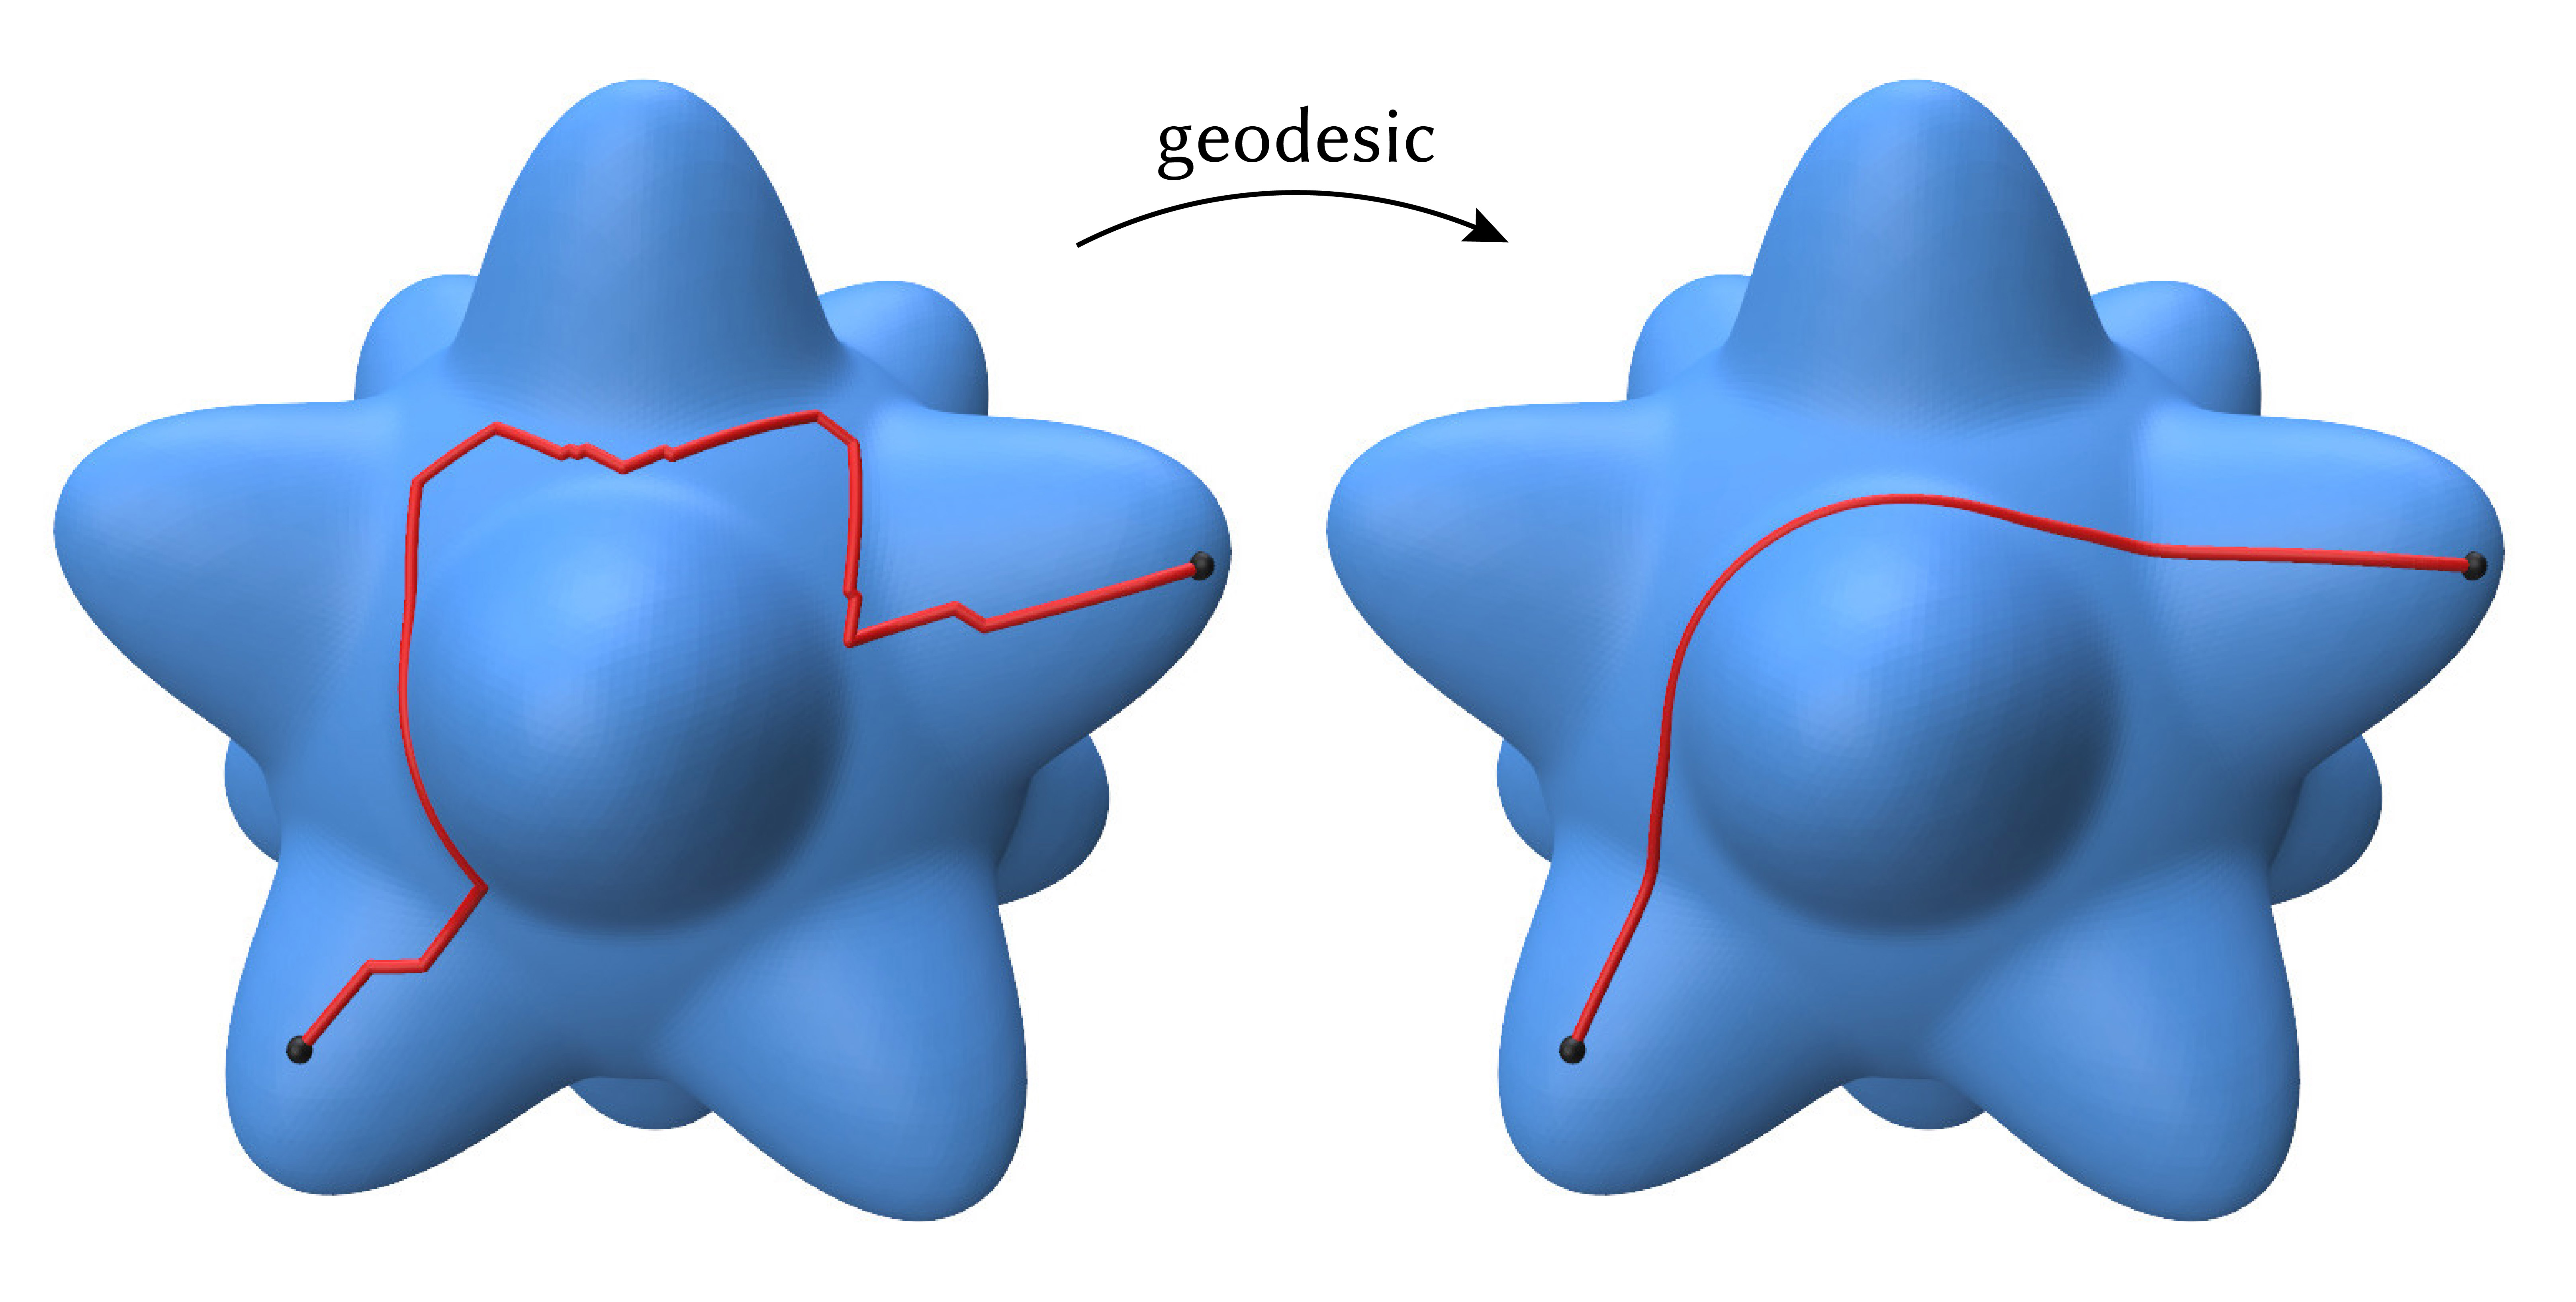
\includegraphics[width=0.6\textwidth]{IMG/flip_geodesic.png}
    \caption{{\bf Geodesic}: It is a curve representing in some sense the shortest path (arc) between two points in a surface.}
    \label{fig:geodesic}
\end{figure}

Geodesics equations can be derived through various concepts like, Equivalence principle, Least action
principle, Parallel transport, etc.

\section*{Derivation from the Equivalence Principle}
The equivalence principle states that the laws of physics are the same for all observers, regardless of their state of motion. This principle can be used to derive the geodesic equation.

{\bf Assume} that a free falling particle is not accelerating in the neighborhood of a point-event with respect to a freely falling coordinate system $X^\mu$. Here the local time $t$ and the three cartesian coordinates $x$, $y$, and $z$ are obtained by substituting $\mu$ with 0, 1, 2, and 3, respectively. So $t=X^0/c$ and
with this assumption, following relation can be written
\begin{equation}
    \frac{d^2X^\mu}{dt^2} = 0
\end{equation}
Which is equivalent to saying that the acceleration is zero. Using multi-dimensional chain rule, above
differential equation can be written in new coordinate system $x^\nu$ as
\begin{equation}\label{eq:geodesic}
    \frac{d^2X^\mu}{dt^2} = \frac{d^2x^\alpha}{dt^2} \frac{\partial X^{\mu}}{\partial x^{\alpha}} + \frac{dx^\alpha}{dt}\frac{dx^\beta}{dt} \frac{d^2X^{\mu}}{dx^{\alpha}dx^{\beta}}=0
\end{equation}

The acceleration in the new coordinate system $x^\nu$ is obtained by multiplying either sides by $\frac{\partial x^{\nu}}{\partial X^{\mu}}$ given by
\begin{align*}
    \frac{d^2x^\alpha}{dt^2} \frac{\partial X^{\mu}}{\partial x^{\alpha}}\frac{\partial x^{\nu}}{\partial X^{\mu}} + \frac{dx^\alpha}{dt}\frac{dx^\beta}{dt} \frac{d^2X^{\mu}}{dx^{\alpha}dx^{\beta}}\frac{\partial x^{\nu}}{\partial X^{\mu}}&=0\\
    \frac{d^2x^\alpha}{dt^2} \delta_{\alpha\nu} + \frac{dx^\alpha}{dt}\frac{dx^\beta}{dt} \left(\frac{d^2X^{\mu}}{dx^{\alpha}dx^{\beta}}\frac{\partial x^{\nu}}{\partial X^{\mu}}\right)&=0
\end{align*}
The term inside the parenthesis is the Christoffel symbol $\Gamma^\nu_{\alpha\beta}$, so the above equation becomes
\begin{equation}
    \frac{d^2x^\nu}{dt^2}=-\Gamma^\nu_{\alpha\beta}\frac{dx^\alpha}{dt}\frac{dx^\beta}{dt}
\end{equation}

It can be seen that the acceleration in the new coordinate system is not necessarily zero, but is given by the Christoffel symbols.

If the proper time $s$, defined as $s^2=g_{\nu\mu}x^\nu x^\mu$, is used as the parameter of motion, then the above equation becomes
\begin{equation}
    \frac{d^2x^\nu}{ds^2}=-\Gamma^\nu_{\alpha\beta}\frac{dx^\alpha}{ds}\frac{dx^\beta}{ds}
\end{equation}
which is the geodesic equation with proper time $s$ as the parameter of motion.



%------------Body-Ends--------------------
%\bibliography{ref.bib}
%\bibliographystyle{IEEEtran}
\end{document}
